% -*- compile-command: "make HOCKING-PeakSeg-functional-pruning-slides.pdf" -*-
\documentclass{beamer}
\usepackage{tikz}
\usepackage[all]{xy}
\usepackage{amsmath,amssymb}
\usepackage{hyperref}
\usepackage{graphicx}
\usepackage{algorithmic}

\DeclareMathOperator*{\argmin}{arg\,min}
\DeclareMathOperator*{\Lik}{Lik}
\DeclareMathOperator*{\PoissonLoss}{PoissonLoss}
\DeclareMathOperator*{\Peaks}{Peaks}
\DeclareMathOperator*{\Segments}{Segments}
\DeclareMathOperator*{\argmax}{arg\,max}
\DeclareMathOperator*{\maximize}{maximize}
\DeclareMathOperator*{\minimize}{minimize}
\newcommand{\sign}{\operatorname{sign}}
\newcommand{\RR}{\mathbb R}
\newcommand{\ZZ}{\mathbb Z}
\newcommand{\NN}{\mathbb N}

% Set transparency of non-highlighted sections in the table of
% contents slide.
\setbeamertemplate{section in toc shaded}[default][100]
\AtBeginSection[]
{
  \setbeamercolor{section in toc}{fg=red} 
  \setbeamercolor{section in toc shaded}{fg=black} 
  \begin{frame}
    \tableofcontents[currentsection]
  \end{frame}
}

\begin{document}

\title{A linear time algorithm for constrained 
optimal segmentation}

\author{
  Toby Dylan Hocking\\
  toby.hocking@mail.mcgill.ca\\
  joint work with Guillem Rigaill, Paul Fearnhead, 
  Guillaume Bourque}

\date{11 Aug 2016}

\maketitle

\section{Problem: optimizing ChIP-seq peak detection}

\begin{frame}
  \frametitle{Chromatin immunoprecipitation sequencing (ChIP-seq)}
  Analysis of DNA-protein interactions.

  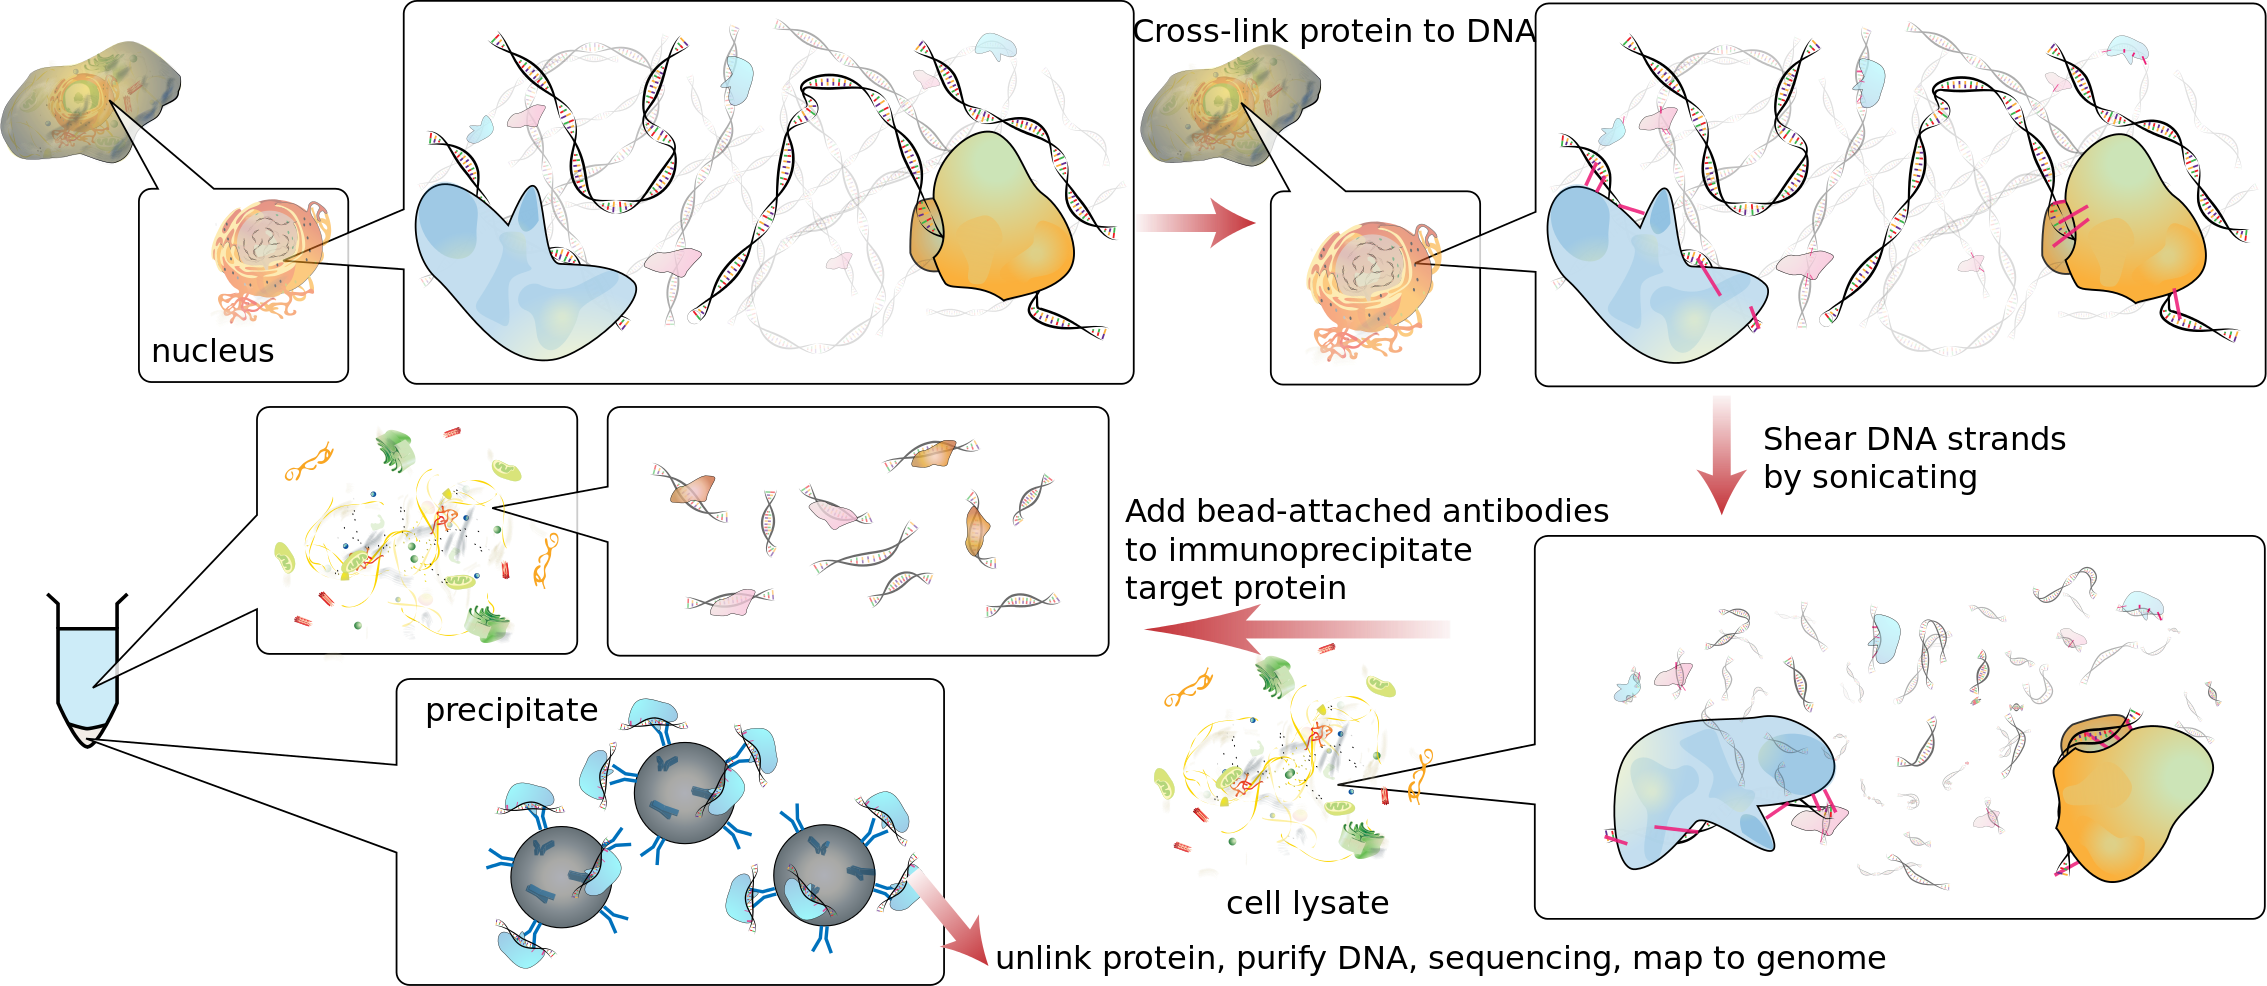
\includegraphics[width=\textwidth]{Chromatin_immunoprecipitation_sequencing_wide.png}

  Source: ``ChIP-sequencing,'' Wikipedia.
\end{frame}

\begin{frame}
  \frametitle{Problem: find peaks in each of several samples}
  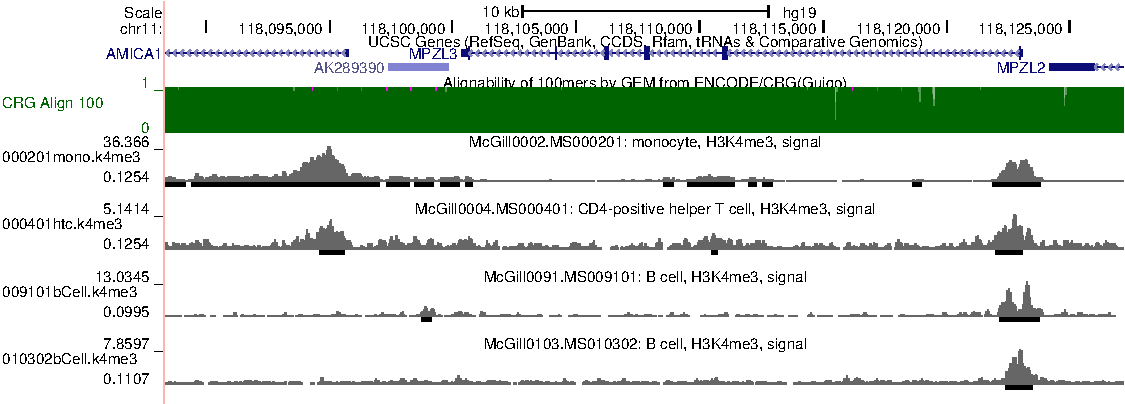
\includegraphics[width=\textwidth]{screenshot-ucsc-edited}

  Grey profiles are normalized aligned read count signals.

  Black bars are ``peaks'' called by MACS2 (Zhang et al, 2008):
  \begin{itemize}
  \item \alert<1>{many false positives}.
  \item overlapping peaks have different start/end positions.
  \end{itemize}
\end{frame}

\begin{frame}
  \frametitle{Previous work in genomic peak detection}
  \begin{itemize}
  \item Model-based analysis of ChIP-Seq (MACS), Zhang et al, 2008.
  \item SICER, Zang et al, 2009.
  \item HOMER, Heinz et al, 2010.
  \item CCAT, Xu et al, 2010.
  \item RSEG, Song et al, 2011.
  \item Triform, Kornacker et al, 2012.
  \item Histone modifications in cancer (HMCan), Ashoor et al, 2013.
  \item PeakSeg, Hocking, Rigaill, Bourque, ICML 2015.
  \item PeakSegJoint Hocking and Bourque, arXiv:1506.01286.
  \item ... dozens of others.
  \end{itemize}
  Two big questions: how to choose the best...
  \begin{itemize}
  \item ...algorithm? (testing)
  \item \alert<1>{...parameters? (training)}
  \end{itemize}
\end{frame}

\begin{frame}[fragile]
  \frametitle{How to choose parameters of unsupervised peak
    detectors?}
\scriptsize
19 parameters for Model-based analysis of ChIP-Seq (MACS), Zhang et al, 2008.
\begin{verbatim}
  [-g GSIZE]
  [-s TSIZE] [--bw BW] [-m MFOLD MFOLD] [--fix-bimodal]
  [--nomodel] [--extsize EXTSIZE | --shiftsize SHIFTSIZE]
  [-q QVALUE | -p PVALUE | -F FOLDENRICHMENT] [--to-large]
  [--down-sample] [--seed SEED] [--nolambda]
  [--slocal SMALLLOCAL] [--llocal LARGELOCAL]
  [--shift-control] [--half-ext] [--broad]
  [--broad-cutoff BROADCUTOFF] [--call-summits]
\end{verbatim}
10 parameters for Histone modifications in cancer (HMCan),
Ashoor et al, 2013.
\begin{verbatim}
minLength 145
medLength 150
maxLength 155
smallBinLength 50
largeBinLength 100000
pvalueThreshold 0.01
mergeDistance 200
iterationThreshold 5
finalThreshold 0
maxIter 20
\end{verbatim}
\end{frame}

\begin{frame}
  \frametitle{Which macs parameter is best for these data?}
  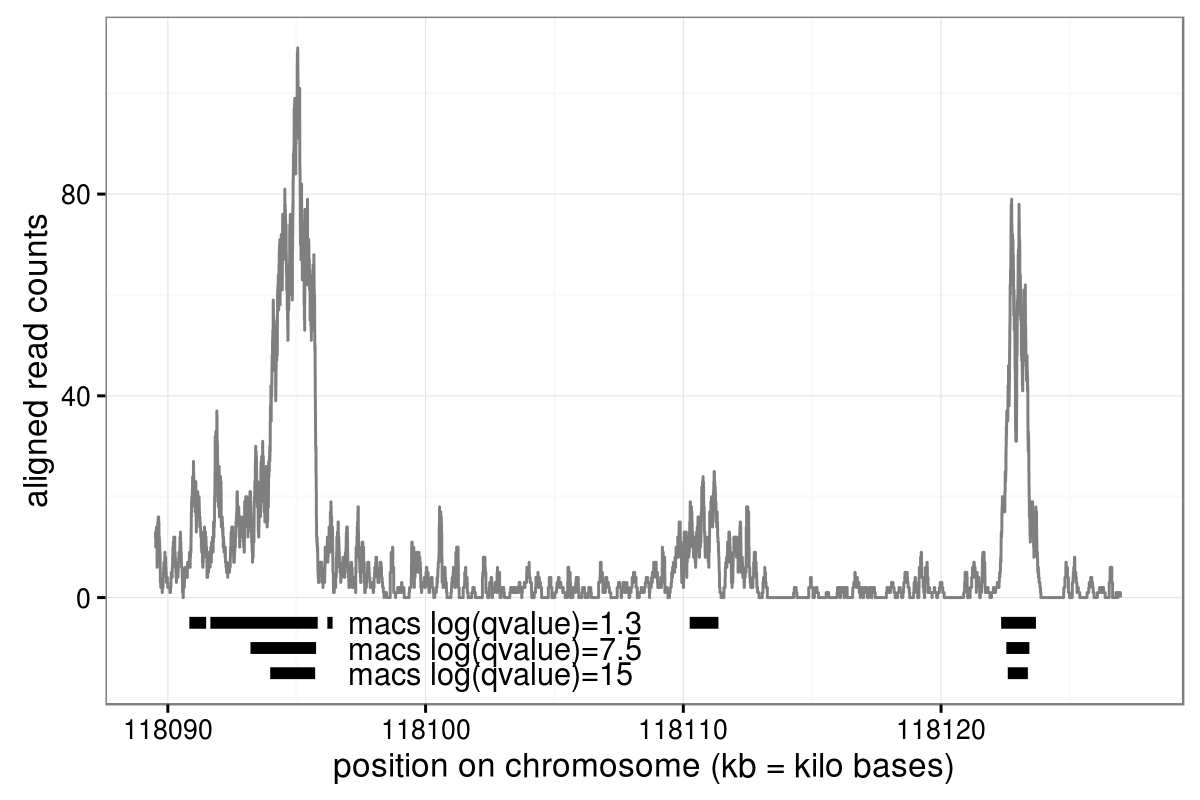
\includegraphics[width=1\textwidth]{figure-macs-problem.png}
\end{frame}

% \begin{frame}
%   \frametitle{Compute likelihood/loss of piecewise constant model}
%   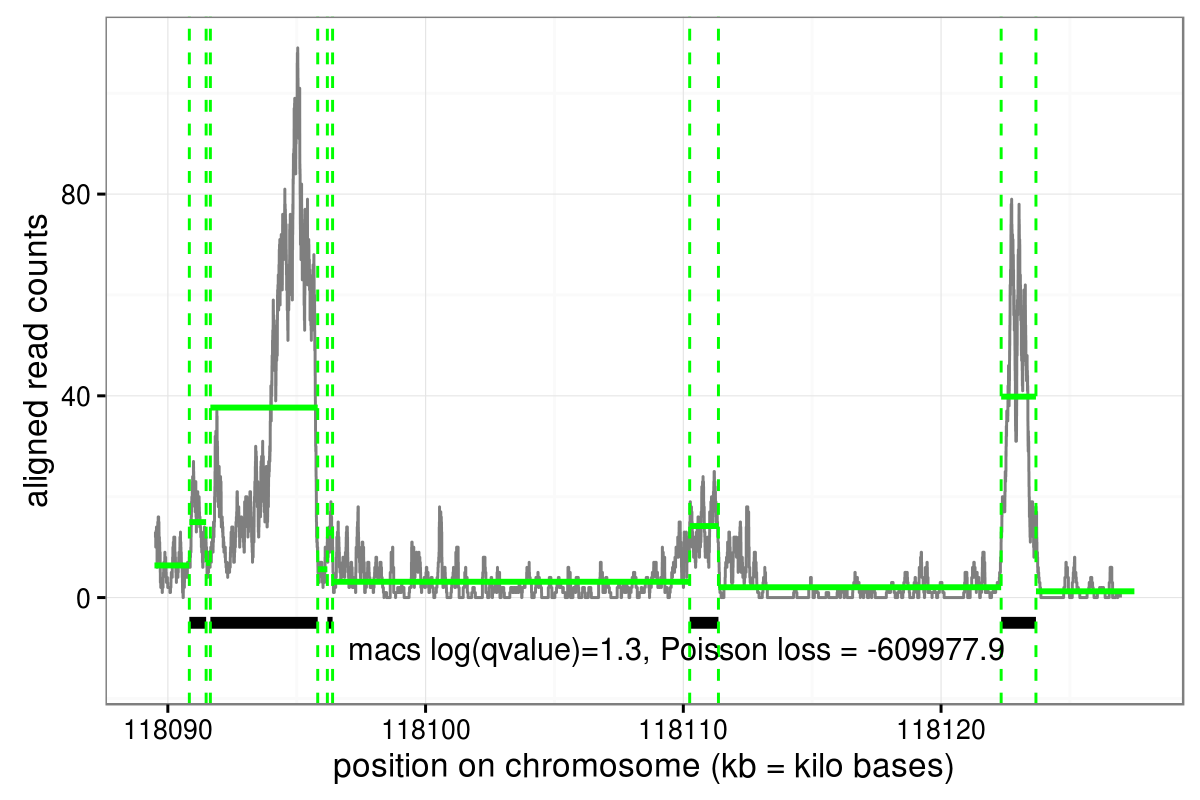
\includegraphics[width=1\textwidth]{figure-macs-problem-1-30103.png}
% \end{frame}

\begin{frame}
  \frametitle{Compute likelihood/loss of piecewise constant model}
  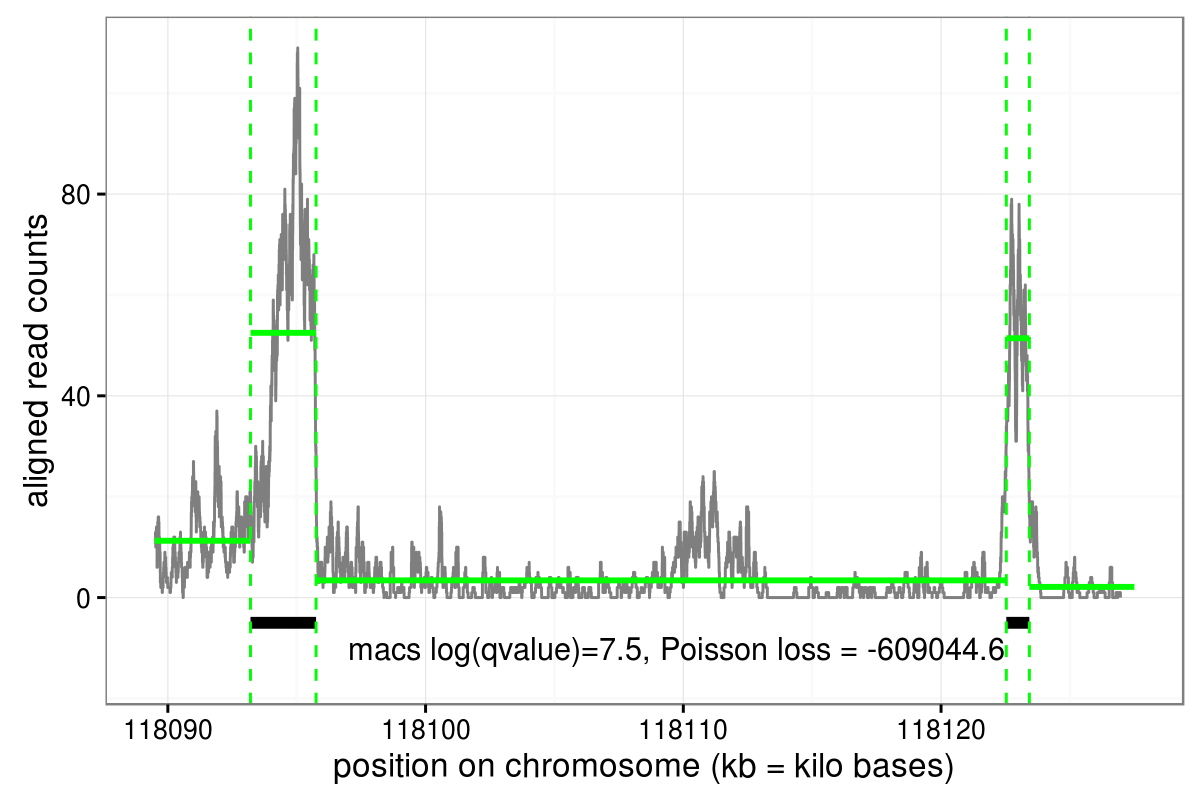
\includegraphics[width=1\textwidth]{figure-macs-problem-7-5.png}
  % $\PoissonLoss(\mathbf z, \mathbf m) = \sum_{i=1}^n m_i - z_i \log(m_i)$
  % for count data $\mathbf z\in\ZZ_+^n$ 
  % and segment mean model $\mathbf m\in\RR^n$.
\end{frame}

\begin{frame}
  \frametitle{Idea: choose the parameter with a lower loss}
  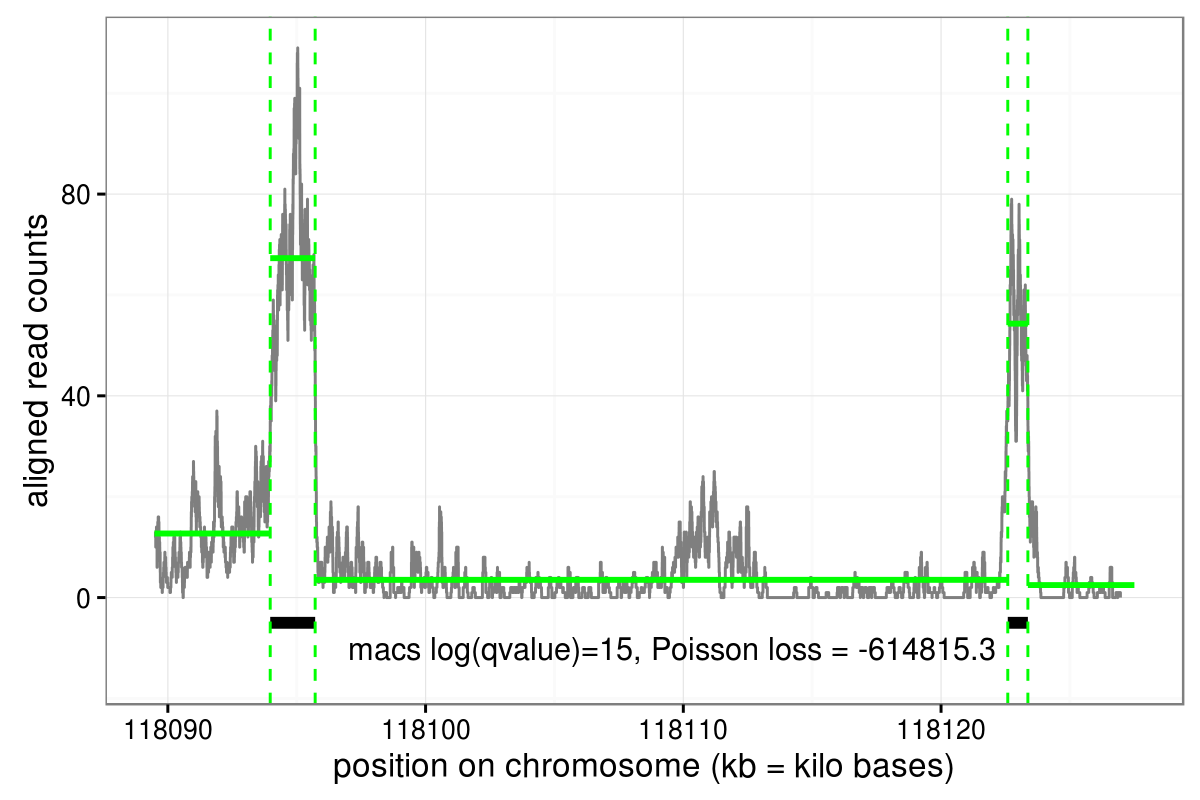
\includegraphics[width=1\textwidth]{figure-macs-problem-15.png}
\end{frame}

\begin{frame}
  \frametitle{PeakSeg: search for the peaks with lowest loss}
  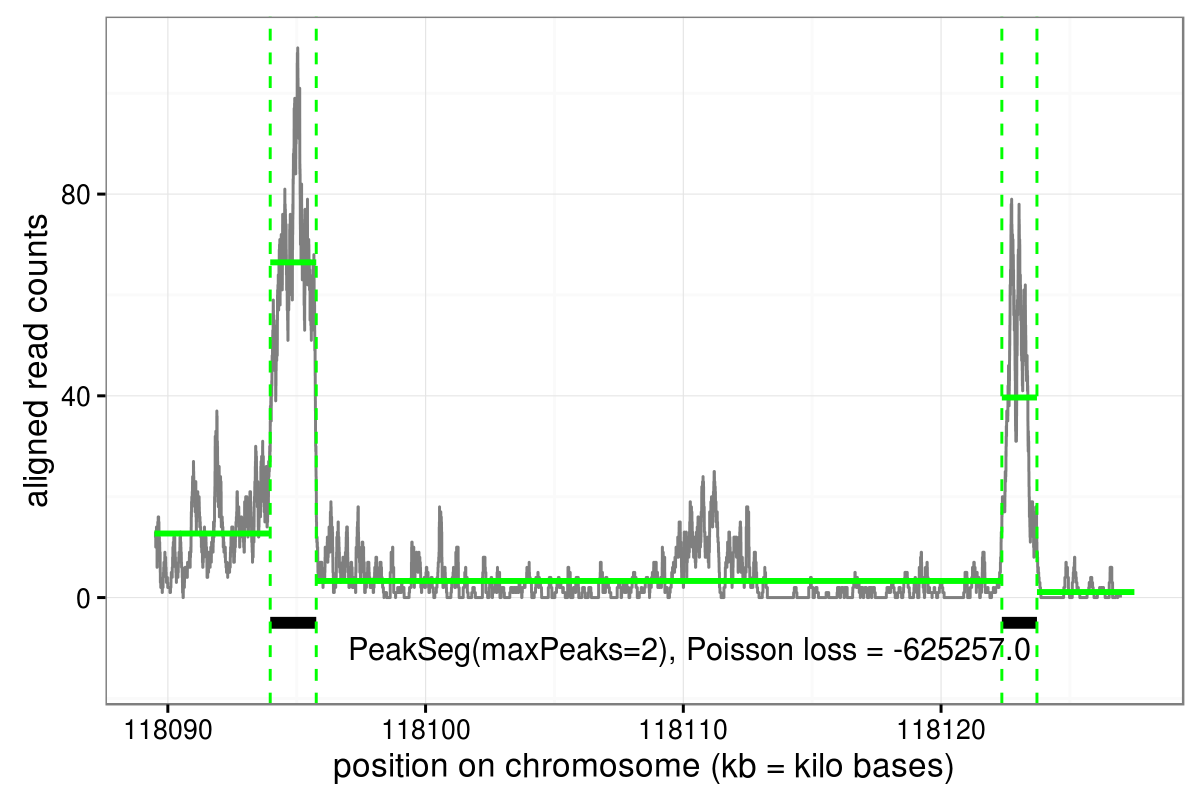
\includegraphics[width=1\textwidth]{figure-macs-problem-PeakSeg.png}
  
  Simple model with only one parameter to train (maxPeaks).
\end{frame}

\begin{frame}
  \frametitle{Maximum likelihood Poisson segmentation models}
  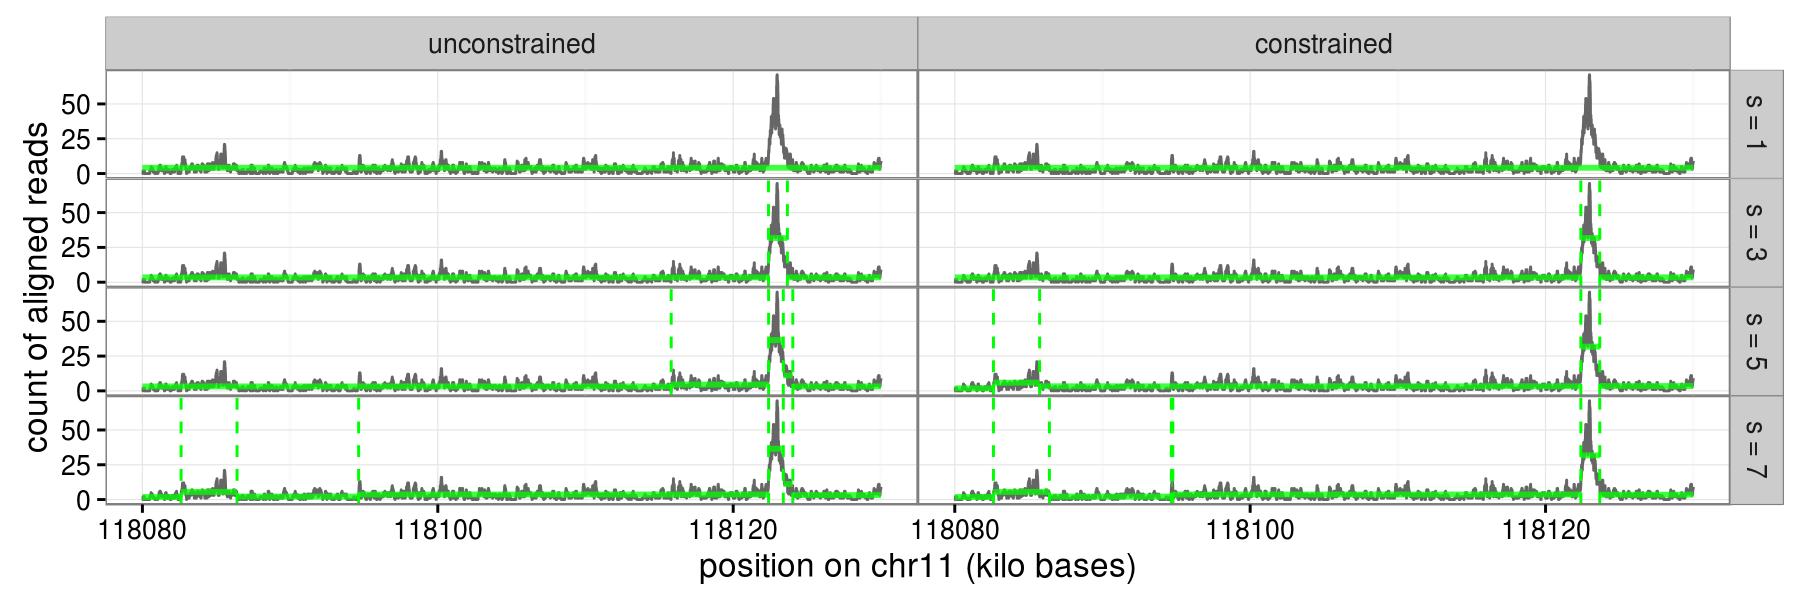
\includegraphics[width=1\textwidth]{figure-Segmentor-PeakSeg}

  \begin{itemize}
  \item Previous work: unconstrained maximum likelihood mean\\
    for $s$ segments ($s-1$ changes).
  \item Hocking et al, ICML 2015: PeakSeg constraint enforces up, down, up,
    down (and not up, up, down). 
  \item Odd-numbered segments are background noise,\\
    even-numbered segments are peaks.
  \item Constrained Dynamic Programming Algorithm, $O(N^2)$ time for $N$ data points.
  \end{itemize}
\end{frame}

\begin{frame}
  \frametitle{But quadratic time is not fast enough for genomic data!}
  \includegraphics[width=\textwidth]{figure-PDPA-timings-dp}
  \begin{itemize}
  \item Genomic data is large, $N \geq 10^6$.
  \item Split into subsets? What if we split a peak in half?
  \item Need linear time algorithm for analyzing whole data set.
  \end{itemize}
\end{frame}

\section{New linear time algorithm using functional pruning}

\begin{frame}
  \frametitle{Relation to previous work}
  \begin{tabular}{r|c|c}
    & no pruning & functional pruning \\
    \hline
    unconstrained & \alert<1>{Dynamic Programming} & \alert<2>{Pruned DP} \\
     & \alert<1>{exact $O(N^2)$} & \alert<2>{exact $O(N\log N)$}\\
    R pkgs: & \alert<1>{changepoint} & \alert<2>{cghseg, Segmentor}\\
    \hline
    up-down constrained & \alert<3>{constrained DP} & \alert<4>{\textbf{this work}} \\
     & \alert<3>{inexact $O(N^2)$} & \alert<4>{exact $O(N\log N)$}\\
    R pkgs: & \alert<3>{PeakSegDP} & \alert<4>{coseg}\\
    \hline
  \end{tabular}
  \begin{itemize}
  \item \alert<1>{Auger and Lawrence 1989, Jackson et al 2005}.
  \item \alert<2>{Rigaill 2010, Johnson 2013, Cleynen et al 2014}.
  \item \alert<3>{Hocking, Rigaill, Bourque 2015}.
  \item \alert<4>{\textbf{Contribution}: new algorithm that
      \textbf{exactly} computes the \textbf{constrained} optimal
      segmentation for $N$ data points in linear $O(N\log N)$ time}.
  \end{itemize}
\end{frame}

% \begin{frame}
%   \frametitle{TODO: difference with unconstrained PDPA figure
%     (min-less function vs min constant)}
% \end{frame}

\begin{frame}
  \frametitle{Functional pruning idea}
  Instead of computing the matrix of optimal loss in $S$ segments up
  to $N$ data points,
$$
\begin{array}{ccc}
  \mathcal L_{1,1} & \cdots &   \mathcal L_{1,N}\\
  \vdots &  & \vdots\\
  \mathcal L_{S,1} & \cdots & \mathcal L_{S,N}\\
\end{array}
$$
We compute a matrix of loss \textbf{functions}
$$
\begin{array}{ccc}
   L_{1,1}(\mu_1) & \cdots & L_{1,N}(\mu_1)\\
  \vdots &  & \vdots\\
   L_{S,1}(\mu_S) & \cdots & L_{S,N}(\mu_S),\\
\end{array}
$$
the optimal loss up to $N$ data points if segment $S$ has mean
$\mu_S$.
\end{frame}

\begin{frame}
  \frametitle{First segment, first data point}
  \begin{itemize}
  \item   For data $z_1, \dots, z_N\in\ZZ_+$ let
  \begin{equation*}
    \gamma_t(\mu) = \mu - z_t \log \mu
  \end{equation*}
  be the Poisson loss for each $t\in\{1, \dots, N\}$.
\item For example $z = 2, 1, 9, 5, 10, 3$.
\item Then $\gamma_1(\mu)=L_{1,1}(\mu)= 1\mu - 2\log \mu + 0$.
\item Need to store 3 coefficients (linear, log, constant).
  \end{itemize}
  \begin{center}
    \includegraphics[width=0.7\textwidth]{figure-PeakSegPDPA-demo-cost-1segments-1data}
  \end{center}
\end{frame}

\begin{frame}
  \frametitle{First segment, other data points}
  \begin{itemize}
\item
  The loss of the first segment up to data point $t$ is
  \begin{equation*}
    \label{eq:C1b}
    L_{1,t}(\mu) = \sum_{i=1}^t \gamma_i(\mu).
  \end{equation*}
\item For example $z = 2, 1, 9, 5, 10, 3$.
% \item $L_{1,2}(\mu) = (2\mu - 3\log\mu + 0)/2 = 1\mu - 1.5\log\mu + 0$.
% \item $L_{1,3}(\mu) = (3\mu - 13\log\mu + 0)/3 = 1\mu - 4.333\log\mu + 0$.
\item $L_{1,2}(\mu) = 2\mu - 3\log\mu + 0$.
\item $L_{1,3}(\mu) = 3\mu - 12\log\mu + 0$.
\item ...
  \end{itemize}
  \begin{center}
    \includegraphics[width=0.5\textwidth]{figure-PeakSegPDPA-demo-cost-1segments-2data}
    \includegraphics[width=0.5\textwidth]{figure-PeakSegPDPA-demo-cost-1segments-3data}
  \end{center}
\end{frame}

\begin{frame}[fragile]
  \frametitle{Second segment, up to data point 2}
  \begin{itemize}
  \item The mean cost in 2 segments up to data point 2 is
\begin{eqnarray*}
  L_{2,2}(\mu_2) 
  &=&  \gamma_2(\mu_2)+\min_{\mu_1 \leq \mu_2} L_{1,1}(\mu_1)\\
  &=& \gamma_2(\mu_2)+L_{1,1}^{\leq}(\mu_2)
\end{eqnarray*}
\item Min-less operator is $L^\leq(\mu) = \min_{x\leq\mu} L(x),$
    \begin{center}
      \includegraphics[width=0.5\textwidth]{figure-PeakSegPDPA-demo-minlessmore-2segments-2data}
    \end{center}
\end{itemize}
\end{frame}

\begin{frame}
  \frametitle{Comparison with unconstrained Pruned DPA}
  \begin{itemize}
  \item For our constrained algorithm, the first segment mean must be
    less than the second, and the first segment cost is a function:
    \begin{equation*}
      L_{2,2}(\mu_2) = \gamma_2(\mu_2)+
      \underbrace{\min_{\mu_1 \leq \mu_2} L_{1,1}(\mu_1)}_{L^\leq_{1,1}(\mu_2)}.
    \end{equation*}
  \item For the unconstrained algorithm, it is \alert<1>{constant}:
    \begin{equation*}
      \widehat{L}_{2,2}(\mu_2) = \gamma_2(\mu_2)+
      \alert<1>{\underbrace{\min_{\mu_1} L_{1,1}(\mu_1)}_{\mathcal L_{1,1}}}.
    \end{equation*}
  \item For example $z = 2, 1, 9, 5, 10, 3$.
    \begin{center}
      \includegraphics[width=0.5\textwidth]{figure-PeakSegPDPA-demo-mincompare-2segments-2data}
    \end{center}
  \end{itemize}
\end{frame}

\begin{frame}
  \frametitle{Storage as a piecewise function on intervals}
  \begin{itemize}
  \item For example $z = 2, 1, 9, 5, 10, 3$.
    \begin{center}
      \includegraphics[width=0.5\textwidth]{figure-PeakSegPDPA-demo-minlessmore-2segments-2data}
    \end{center}
  \item Storage: 
    \begin{equation*}
      L_{2,2}(\mu) = \gamma_2(\mu) + 
      \begin{cases}
        L_{1,1}(\mu) = 1\mu - 2\log \mu + 0 & \text{ if } \mu\in[1,2],\\
        \mathcal L_{1,1} = 0\mu -0\log\mu + 0.6137 & \text{ if } \mu\in[2,14].
      \end{cases}
    \end{equation*}
  \end{itemize}
\end{frame}

 
\begin{frame}[fragile]
  \frametitle{Second segment, up to data point 3}
  \begin{itemize}
  \item For data point 3 we need to consider two change-points:
    \begin{equation*}
      L_{2,3}(\mu) =  \gamma_3(\mu) + \min
      \begin{cases}
        L_{1,2}^{\leq}(\mu), & \text{ change up after data point 2},\\
        L_{2,2}(\mu), & \text{ change up after data point 1}. 
      \end{cases}
    \end{equation*}
  \item For $z = 2, 1, 9, 5, 10, 3$ the min operation prunes a
    change after data point 1.
    \begin{center}
      \includegraphics[width=0.5\textwidth]{figure-PeakSegPDPA-demo-minenv-2segments-3data}
    \end{center}
  \end{itemize}
\end{frame}

\begin{frame}
  \frametitle{Second segment, up to data point t}
  \begin{itemize}
  \item The updates continue for every data point $t\in\{3, ..., N\}$
    \begin{equation*}
      L_{2,t}(\mu) =  \gamma_t(\mu) + \min
      \begin{cases}
        L_{2,t-1}(\mu),\\
        L_{1,t-1}^{\leq}(\mu).
      \end{cases}
    \end{equation*}
  \item For example for $z = 2, 1, 9, 5, 10, 3$, at data point $t=4$
    we only need to consider changes after 2 and 3 (1 has been
    pruned).
    \begin{center}
      \includegraphics[width=0.5\textwidth]{figure-PeakSegPDPA-demo-minenv-2segments-4data}
    \end{center}
  \end{itemize}
\end{frame}


\begin{frame}
  \frametitle{Functional pruning complete example}
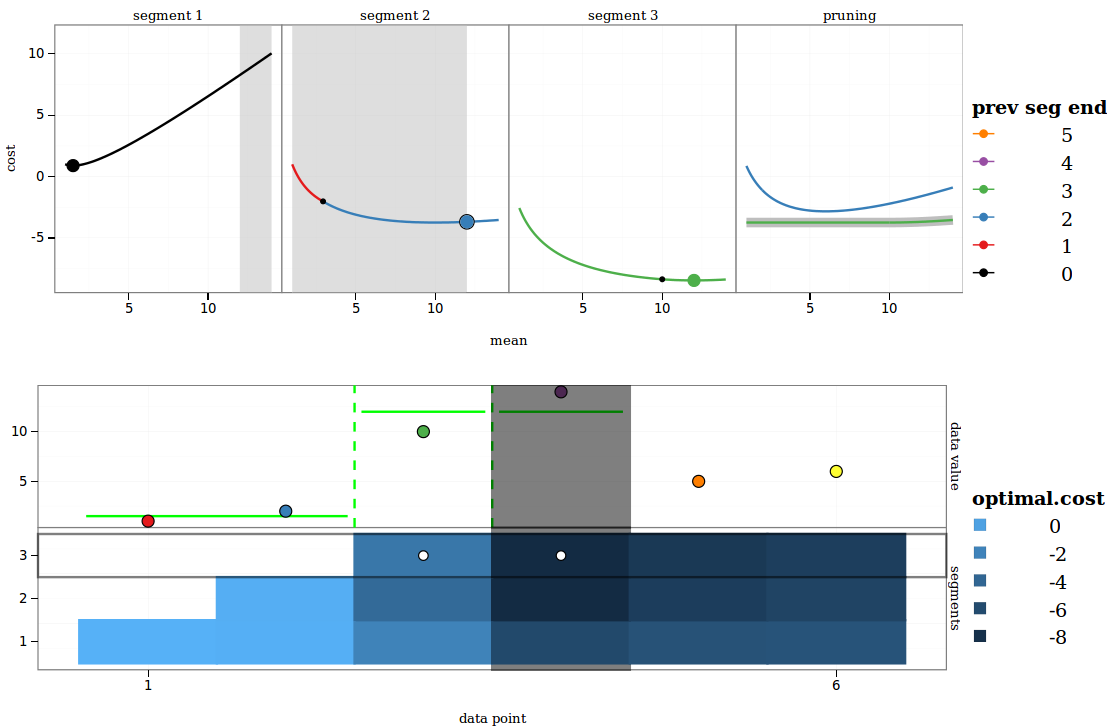
\includegraphics[width=\textwidth]{screenshot-PDPA-demo}

  \url{https://github.com/tdhock/PeakSegFPOP-paper}
  %\url{http://bl.ocks.org/tdhock/raw/8c5dd0af533e24a893e7c5232f9bc94c/}
\end{frame}

\begin{frame}
  \frametitle{General functional pruning equation}
  \begin{itemize}
  \item The constrained cost of a mean $\mu$ for the segment $s$,
    up to data point $t$:
    \begin{equation*}
      L_{s,t}(\mu) = \gamma_t(\mu) + \min
      \begin{cases}
        L_{s,t-1}(\mu),\\
        L_{s-1,t-1}^{*}(\mu),
      \end{cases}
    \end{equation*}
  \item Time complexity of min and min-less/more * is linear in the
    number of intervals, empirically sub-linear $O(\log N)$.
    \includegraphics[width=0.5\textwidth]{figure-PDPA-intervals-all}
  \item Total time complexity: $O(S N\log N)$.
  \end{itemize}
\end{frame}

\section{Interpretation of equal segment means}

\begin{frame}
  \frametitle{What does our solution say about the PeakSeg solution?}
  \begin{itemize}
  \item Our algo exactly solves a problem with \textbf{non-strict
      inequality} constraints.
  \item For example, $N=3$ data points and $S=3$ segments,
    \begin{equation*}
      \min_{\mu_1\leq\mu_2\geq\mu_3}
      \sum_{t=1}^N m_t - z_t\log m_t.
    \end{equation*}
  \item But the PeakSeg problem has \textbf{strict inequality}
    constraints:
    \begin{equation*}
      \min_{\mu_1<\mu_2 >\mu_3}
      \sum_{t=1}^N m_t - z_t\log m_t.
    \end{equation*}
  \end{itemize}
  When our algo returns equal values for adjacent segment means,
  \begin{itemize}
  \item Our solution is not feasible for the PeakSeg problem, and
  \item The PeakSeg solution is undefined.
  \end{itemize}
\end{frame}


\begin{frame}
  \frametitle{Example: 13, 14, 10, 1}
  What do you think is the best model with 1 peak?\\
  (3 segments, 1 change up, 1 change down)
  
  \vskip 1cm

  Guessing game:

  \url{https://github.com/tdhock/PeakSegFPOP-paper/blob/master/figure-min-undefined.R} 
\end{frame}

\begin{frame}
  \frametitle{PeakSegDP returns this highly suboptimal model}
  \includegraphics[width=\textwidth]{figure-min-undefined-suboptimal}
\end{frame}

\begin{frame}
  \frametitle{A better model}
  \includegraphics[width=\textwidth]{figure-min-undefined-1}
\end{frame}

\begin{frame}
  \frametitle{Even better}
  \includegraphics[width=\textwidth]{figure-min-undefined-2}
\end{frame}

\begin{frame}
  \frametitle{Still better}
  \includegraphics[width=\textwidth]{figure-min-undefined-3}
\end{frame}

\begin{frame}
  \frametitle{We can keep going forever}
  \includegraphics[width=\textwidth]{figure-min-undefined-4}
\end{frame}

\begin{frame}
  \frametitle{Best model is not feasible}
  \includegraphics[width=\textwidth]{figure-min-undefined}
\end{frame}

\section{Results on benchmark data set}

\begin{frame}
  \frametitle{Benchmark data, algorithms}

  Data: \url{http://cbio.ensmp.fr/~thocking/chip-seq-chunk-db/}
  \begin{itemize}
  \item 4 annotators (AM, TDH, PGP, XJ).
  \item 8 cell types.
  \item 37 annotated H3K4me3 profiles (sharp peaks).
  \item 29 annotated H3K36me3 profiles (broadly enriched domains).
  \item 2,752 separate segmentation problems.
  \end{itemize}

  Algorithms for segmenting $N$ data points:
  \begin{center}
  \begin{tabular}{ccccc}
    package & constraint & exact? & complexity \\
    \hline
    coseg & $\mu_1 \leq \mu_2 \geq \mu_3 \dots$ & yes & $O(N\log N)$ \\
    PeakSegDP & $\mu_1 < \mu_2 > \mu_3 \dots$ & no & $O(N^2)$\\
    Segmentor & none & yes & $O(N\log N)$
  \end{tabular}

  \vskip 0.5cm

  Segmentor loss $\leq$ coseg loss $\leq$ PeakSegDP loss.
  \end{center}
\end{frame}

\begin{frame}
  \frametitle{Linear time algorithms faster for larger data sets}
  \includegraphics[width=1\textwidth]{figure-PDPA-timings.pdf}

  Total time to compute 10 models (0, ..., 9 peaks) for all data sets:
  \begin{itemize}
  \item PeakSegDP: 156 hours, inexact.
  \item coseg: 6 hours, exact.
  \end{itemize}
\end{frame}

\begin{frame}
  \frametitle{New coseg algorithm more accurate than unconstrained
    maximum likelihood Poisson model (Segmentor)}
  \includegraphics[width=\textwidth]{figure-min-train-error-Segmentor}
\end{frame}

\begin{frame}
  \frametitle{New coseg algorithm mostly agrees with slower inexact DP}
  \includegraphics[width=\textwidth]{figure-min-train-error-PeakSegDP}
\end{frame}

\begin{frame}
  \frametitle{New coseg algorithm sometimes disagrees with macs}
  \includegraphics[width=\textwidth]{figure-min-train-error-macs}
\end{frame}

\begin{frame}
  \frametitle{0 errors for coseg/PeakSegDP, 6 errors for Segmentor}
  \includegraphics[width=\textwidth]{figure-min-train-error-problem2}
\end{frame}

\begin{frame}
  \frametitle{0 errors for coseg/PeakSegDP, 6 errors for Segmentor}
  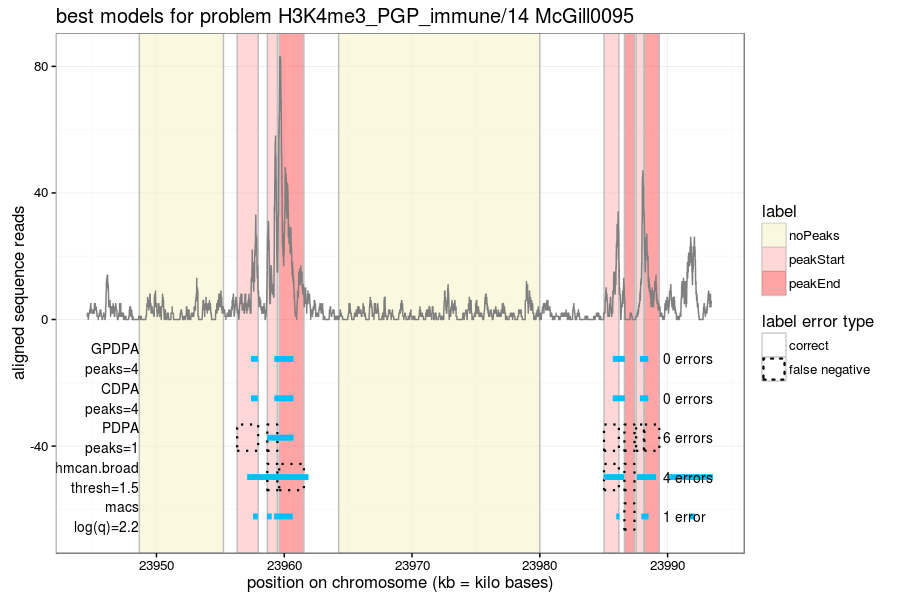
\includegraphics[width=\textwidth]{figure-min-train-error-problem2-best.png}
\end{frame}


% \begin{frame}
%   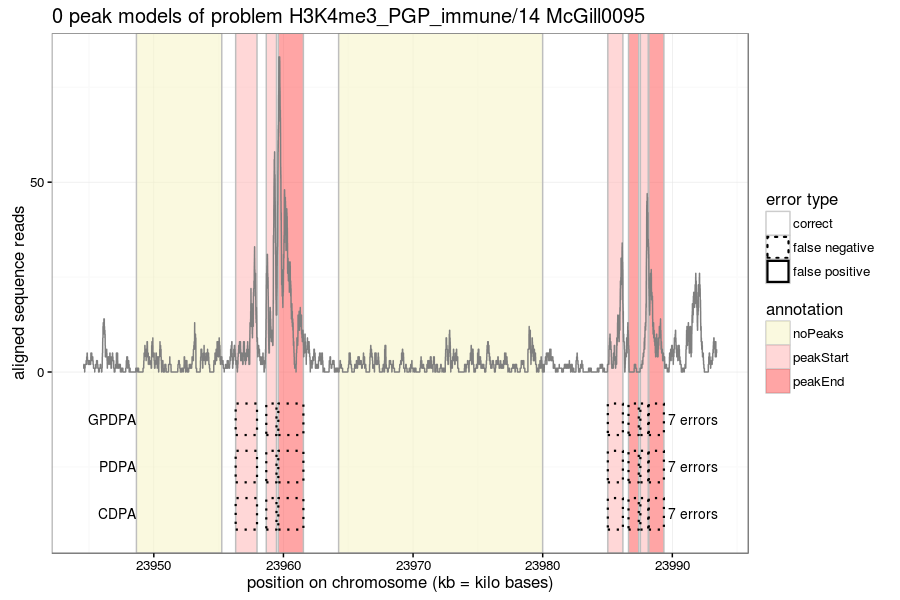
\includegraphics[width=\textwidth]{figure-min-train-error-problem2-0peaks.png}
% \end{frame}

% \begin{frame}
%   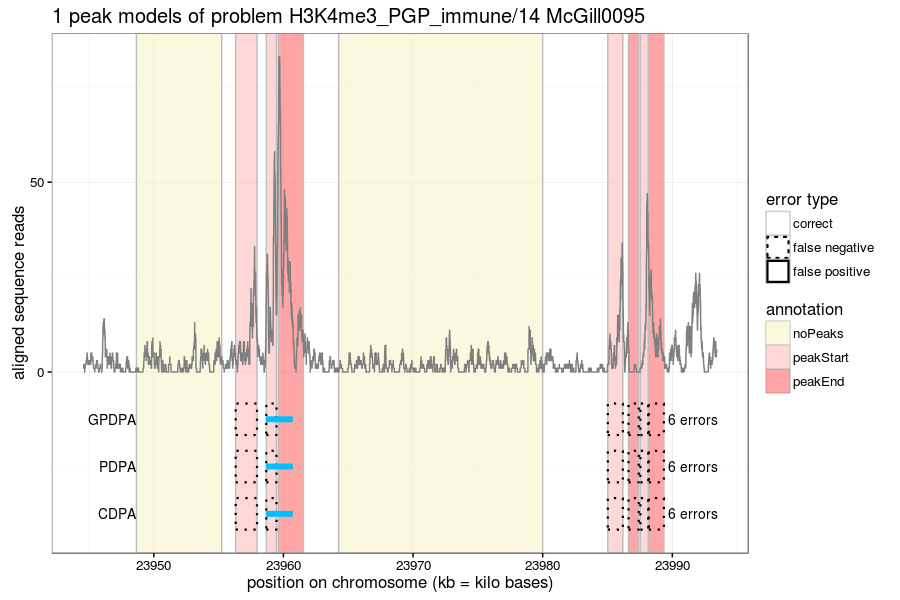
\includegraphics[width=\textwidth]{figure-min-train-error-problem2-1peaks.png}
% \end{frame}

% \begin{frame}
%   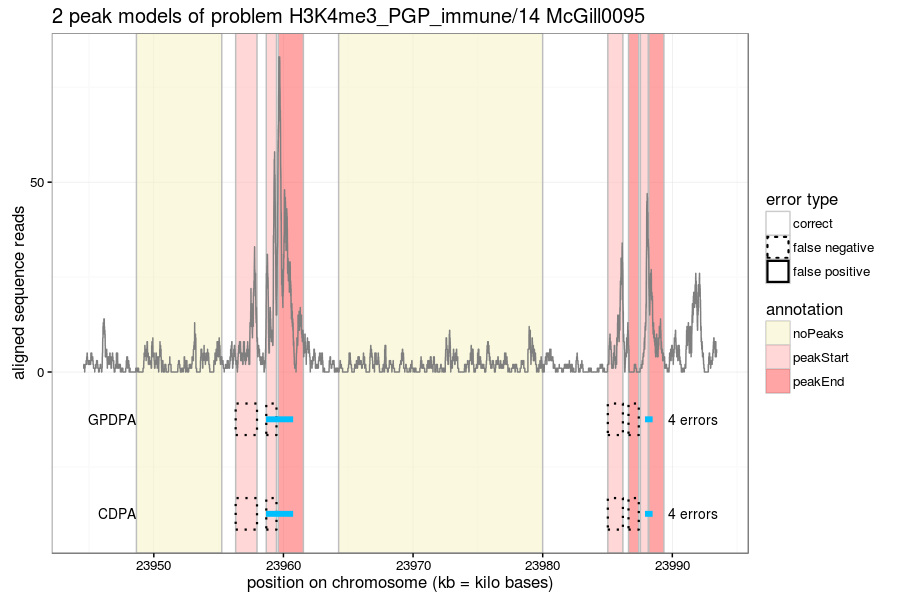
\includegraphics[width=\textwidth]{figure-min-train-error-problem2-2peaks.png}
% \end{frame}

% \begin{frame}
%   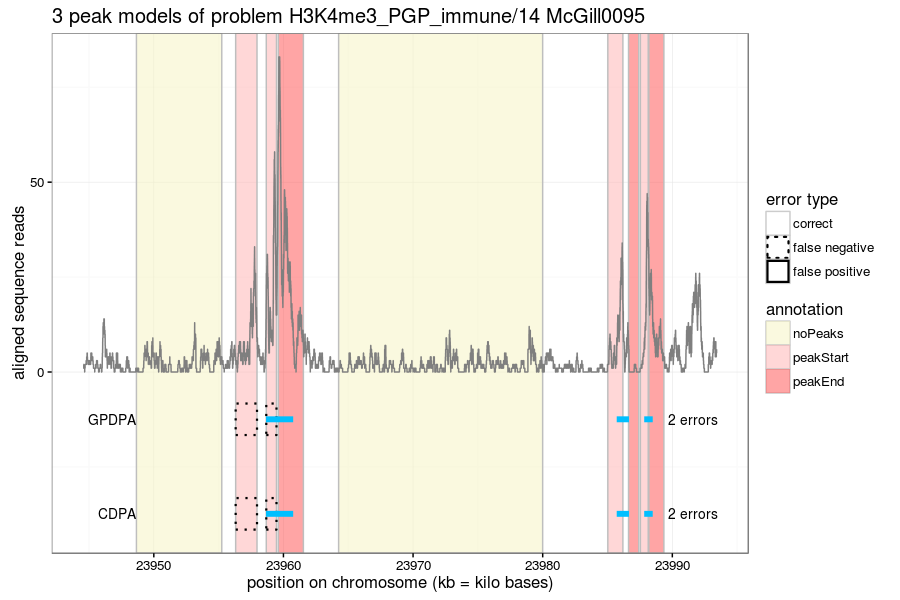
\includegraphics[width=\textwidth]{figure-min-train-error-problem2-3peaks.png}
% \end{frame}

% \begin{frame}
%   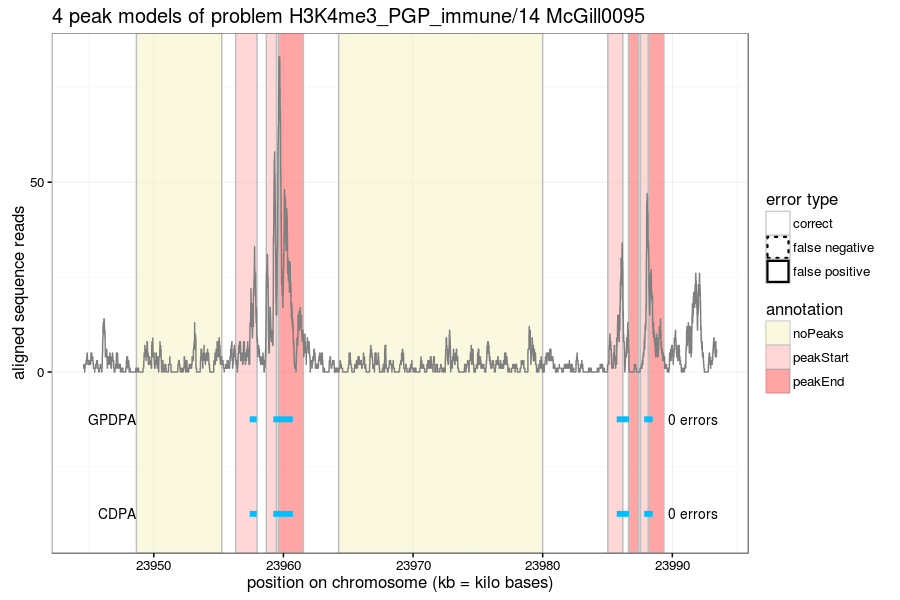
\includegraphics[width=\textwidth]{figure-min-train-error-problem2-4peaks.png}
% \end{frame}

\begin{frame}
  \frametitle{5 errors for coseg/Segmentor, only 1 error for PeakSegDP}
  \includegraphics[width=\textwidth]{figure-min-train-error-problem1}
\end{frame}

\begin{frame}
  \frametitle{5 errors for coseg/Segmentor, only 1 error for PeakSegDP}
  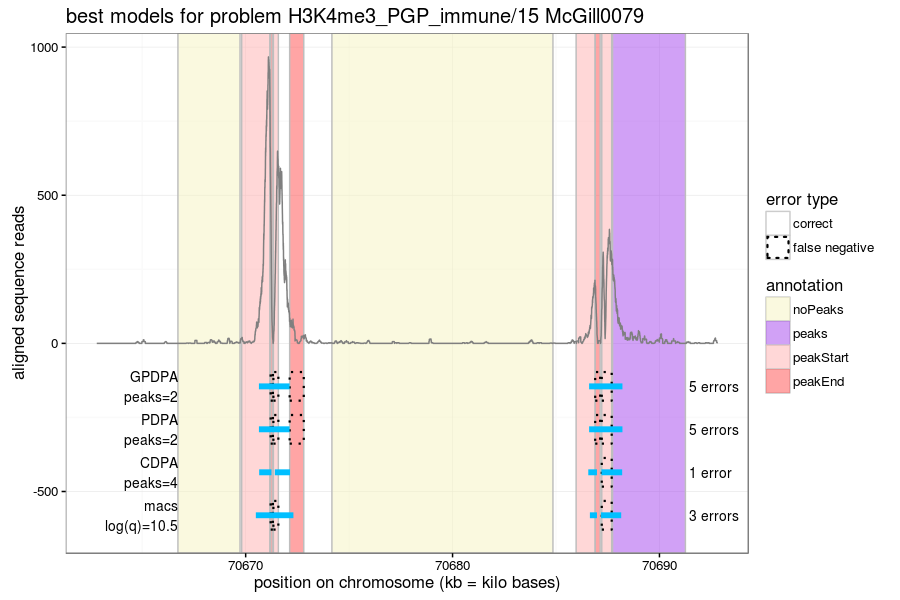
\includegraphics[width=\textwidth]{figure-min-train-error-problem1-best.png}
\end{frame}

% \begin{frame}
%   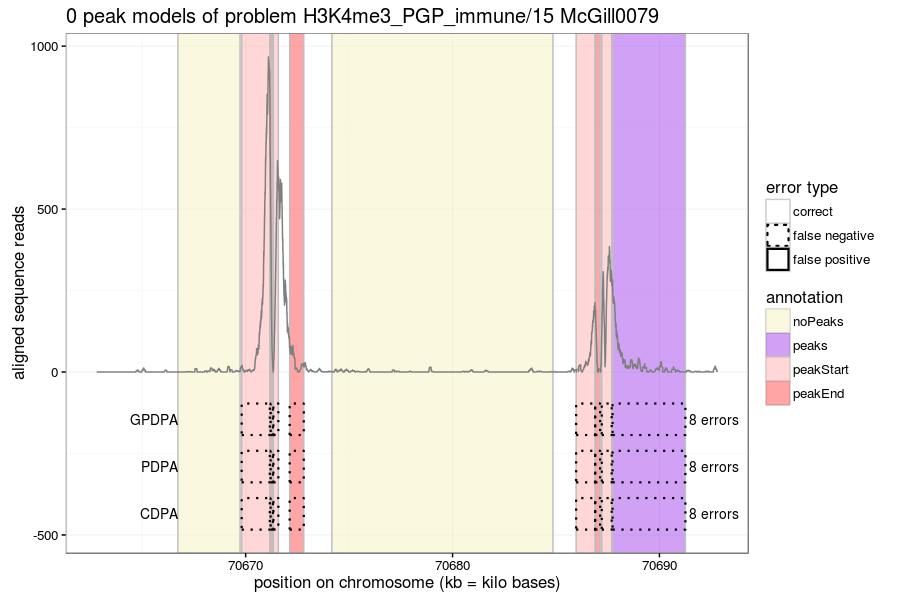
\includegraphics[width=\textwidth]{figure-min-train-error-problem1-0peaks.png}
% \end{frame}

% \begin{frame}
%   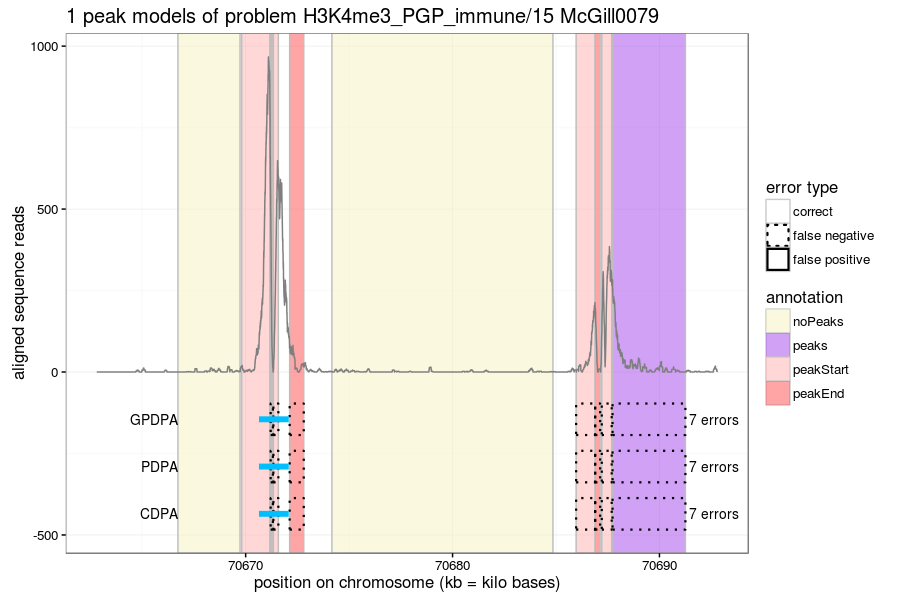
\includegraphics[width=\textwidth]{figure-min-train-error-problem1-1peaks.png}
% \end{frame}

% \begin{frame}
%   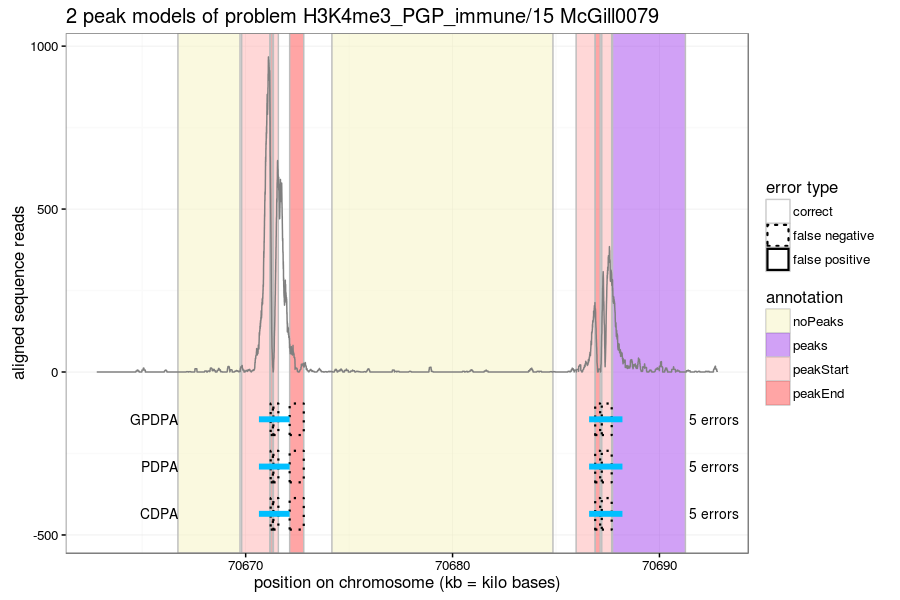
\includegraphics[width=\textwidth]{figure-min-train-error-problem1-2peaks.png}
% \end{frame}

% \begin{frame}
%   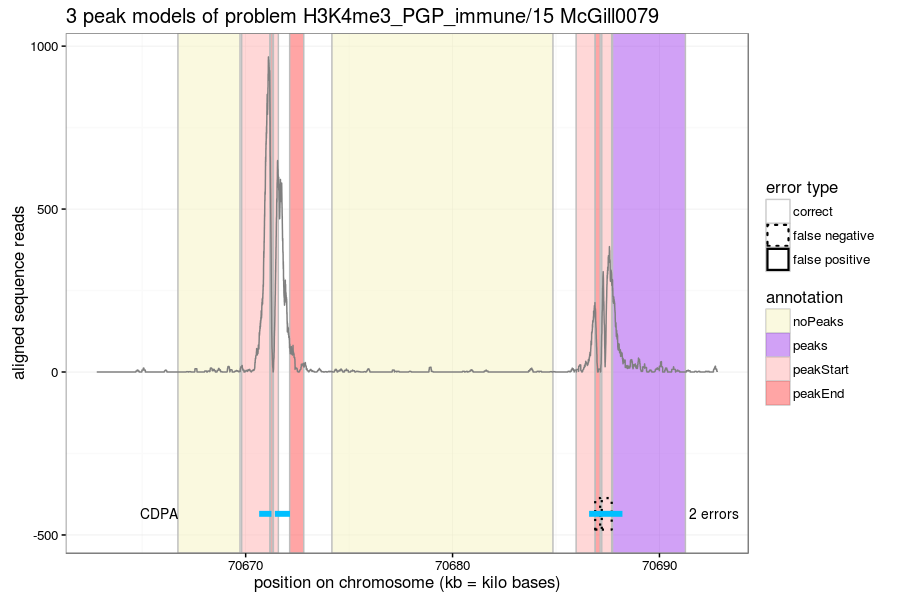
\includegraphics[width=\textwidth]{figure-min-train-error-problem1-3peaks.png}
% \end{frame}

% \begin{frame}
%   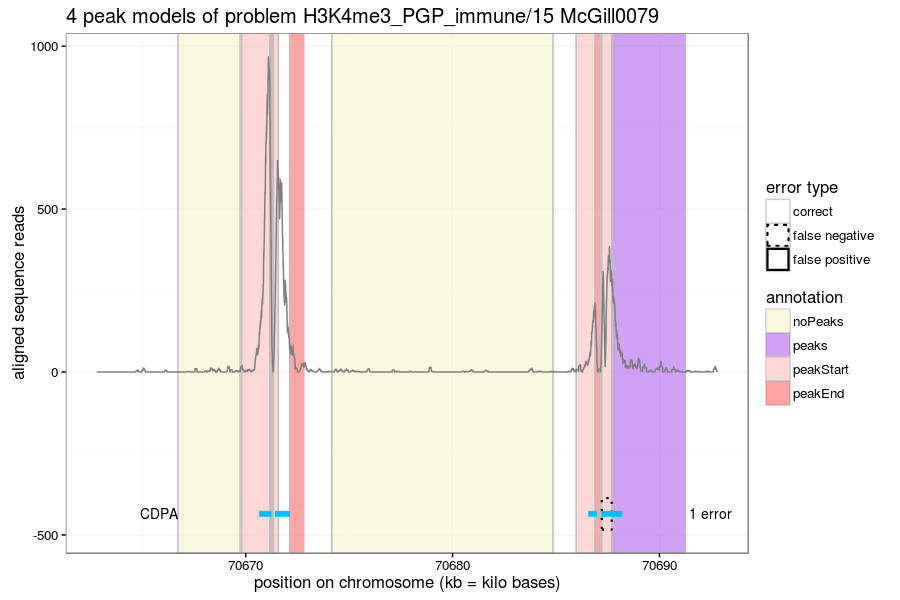
\includegraphics[width=\textwidth]{figure-min-train-error-problem1-4peaks.png}
% \end{frame}

\begin{frame}
  \frametitle{Constrained optimization worse than macs}
  \includegraphics[width=\textwidth]{figure-min-train-error-problem4}
\end{frame}

\begin{frame}
  \frametitle{Constrained optimization worse than macs}
  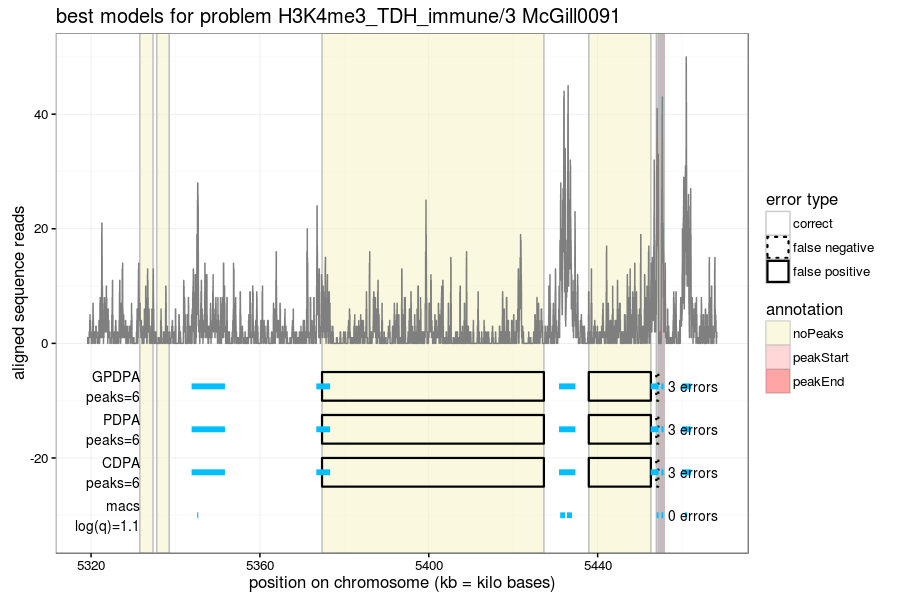
\includegraphics[width=\textwidth]{figure-min-train-error-problem4-best}
\end{frame}

\begin{frame}
  \frametitle{Constrained optimization worse than macs}
  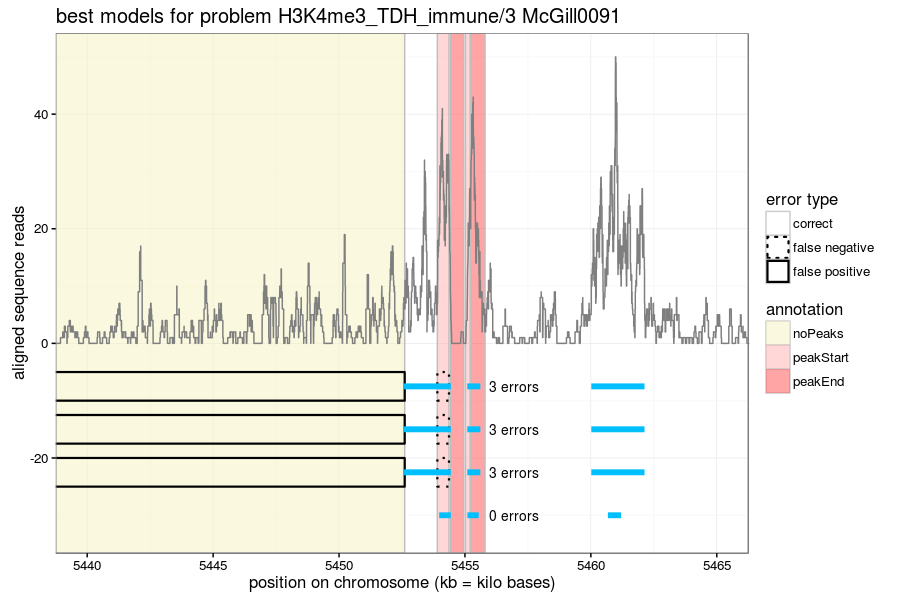
\includegraphics[width=\textwidth]{figure-min-train-error-problem4-best-zoom}
\end{frame}


\begin{frame}
  \frametitle{Constrained optimization better than macs}
  \includegraphics[width=\textwidth]{figure-min-train-error-problem5}
\end{frame}

\begin{frame}
  \frametitle{Constrained optimization better than macs}
  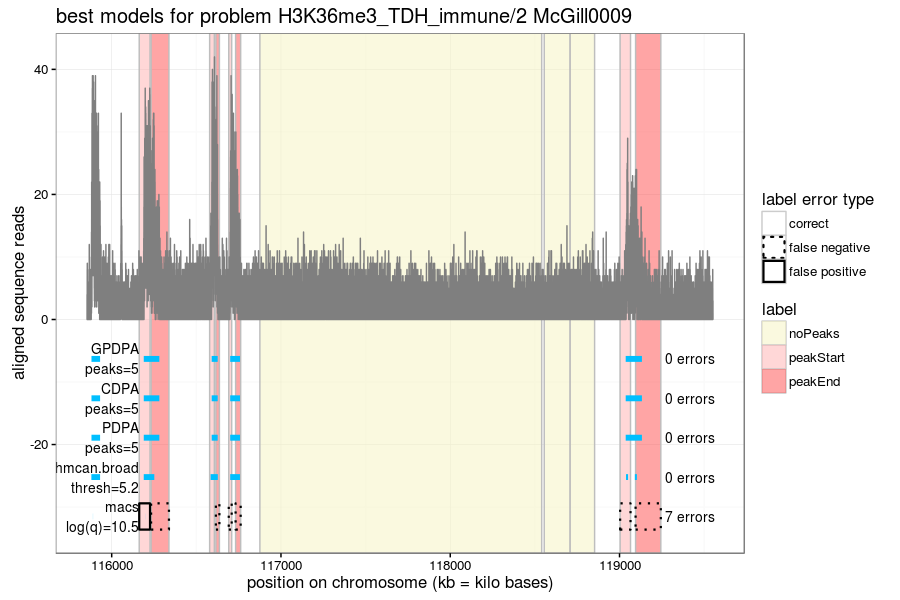
\includegraphics[width=\textwidth]{figure-min-train-error-problem5-best}
\end{frame}

\section{Conclusions and future work}

\begin{frame}[fragile]
  \frametitle{How to choose parameters of unsupervised peak
    detectors?}
\scriptsize
19 parameters for Model-based analysis of ChIP-Seq (MACS), Zhang et al, 2008.
\begin{verbatim}
  [-g GSIZE]
  [-s TSIZE] [--bw BW] [-m MFOLD MFOLD] [--fix-bimodal]
  [--nomodel] [--extsize EXTSIZE | --shiftsize SHIFTSIZE]
  [-q QVALUE | -p PVALUE | -F FOLDENRICHMENT] [--to-large]
  [--down-sample] [--seed SEED] [--nolambda]
  [--slocal SMALLLOCAL] [--llocal LARGELOCAL]
  [--shift-control] [--half-ext] [--broad]
  [--broad-cutoff BROADCUTOFF] [--call-summits]
\end{verbatim}
10 parameters for Histone modifications in cancer (HMCan),
Ashoor et al, 2013.
\begin{verbatim}
minLength 145
medLength 150
maxLength 155
smallBinLength 50
largeBinLength 100000
pvalueThreshold 0.01
mergeDistance 200
iterationThreshold 5
finalThreshold 0
maxIter 20
\end{verbatim}
\end{frame}

\begin{frame}
  \frametitle{Which macs parameter is best for these data?}
  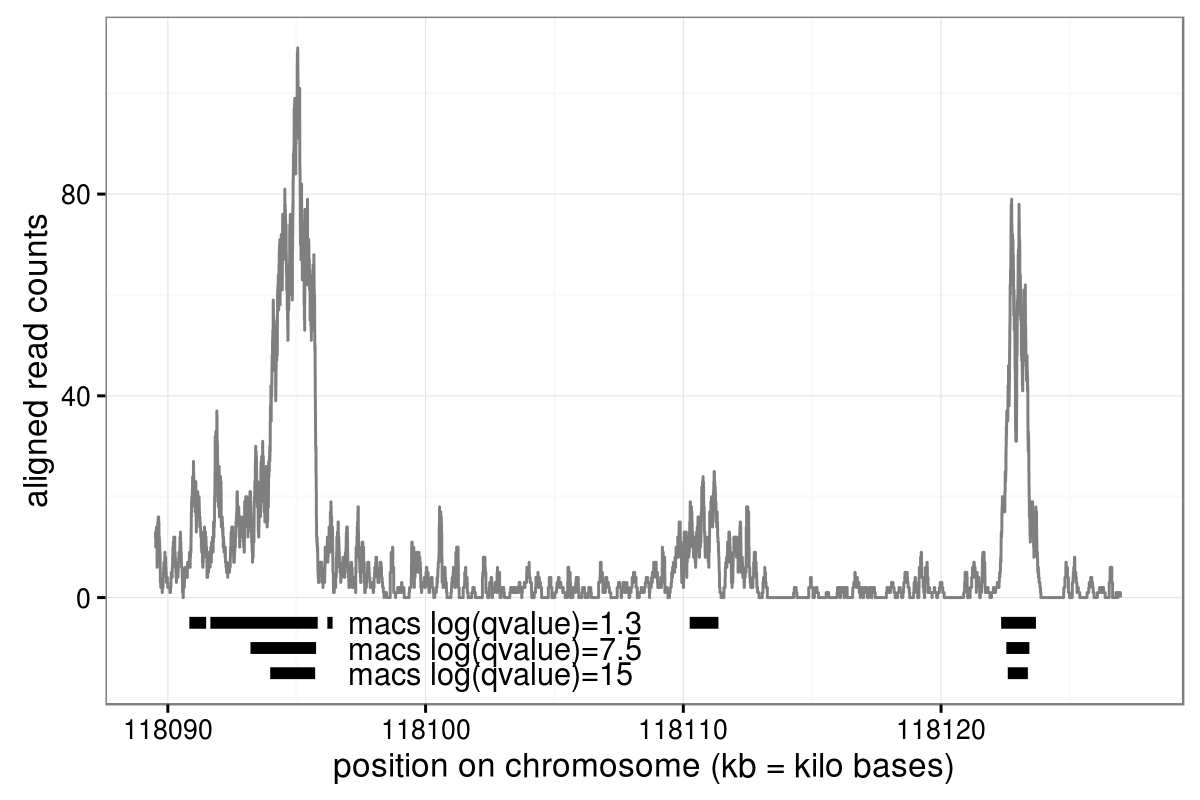
\includegraphics[width=1\textwidth]{figure-macs-problem.png}
\end{frame}

\begin{frame}
  \frametitle{PeakSeg: search for the peaks with lowest loss}
  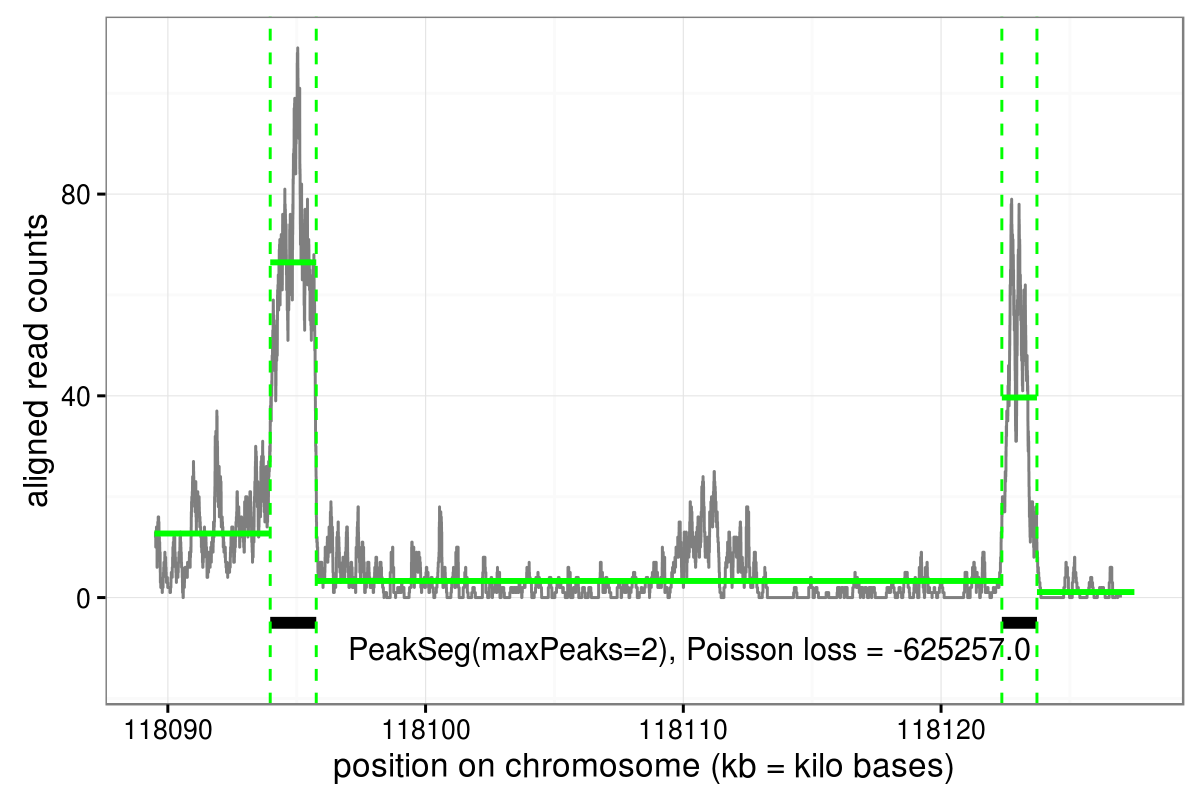
\includegraphics[width=1\textwidth]{figure-macs-problem-PeakSeg.png}
  
  Simple model with only one parameter to train (maxPeaks).
\end{frame}

\begin{frame}
  \frametitle{Conclusions}
  \begin{tabular}{r|c|c}
    & no pruning & functional pruning \\
    \hline
    unconstrained & Dynamic Programming & Pruned DP \\
     & exact $O(N^2)$ & exact $O(N\log N)$\\
    R pkgs: & changepoint & cghseg, Segmentor\\
    \hline
    up-down constrained & constrained DP & \textbf{this work} \\
     & inexact $O(N^2)$ & exact $O(N\log N)$\\
    R pkgs: & PeakSegDP & \textbf{coseg}\\
    \hline
  \end{tabular}
  \begin{itemize}
  \item New algorithm that \textbf{exactly} computes the
    \textbf{constrained} optimal change-points/peaks for $N$ data points.
  \item C++ implementation in coseg R package, 
    \url{https://github.com/tdhock/coseg}
  \item TODO: regularized isotonic regression solver.
  \item TODO: supervised peak calling on entire genomes.
  \end{itemize}
\end{frame}

\begin{frame}
  \frametitle{Segmenting whole chromosomes?}
  \includegraphics[width=\textwidth]{screenshot-gap-peaks}
  \begin{itemize}
  \item 365 regions with no gaps in hg19.
  \item 272 regions with no gaps on chr1-22, X, Y.
  \item Smallest: 31,833 bases (chr6:157,609,467-157,641,300).
  \item Largest: 115,591,997 bases (chr4:75,452,279-191,044,276).
  \end{itemize}
\end{frame}


\begin{frame}
  \frametitle{Reasonable time to segment biggest region on chr1}
  \includegraphics[width=\textwidth]{figure-cosegData-timings.pdf}
  \begin{itemize}
  \item R package in memory: $O(N \log N)$ time.
  \item Command line program on disk: $O(N \log N)$ time.
  \end{itemize}
\end{frame}

\begin{frame}
  \frametitle{Memory requirements reasonable for on-disk version}
  \includegraphics[width=\textwidth]{figure-cosegData-timings-memory-disk.pdf}
  \begin{itemize}
  \item R package in memory: $O(N \log N)$ memory.
  \item Command line program on disk: $O(\log N)$ memory.
  \end{itemize}
\end{frame}

\begin{frame}
  \frametitle{Disk usage reasonable}
  \includegraphics[width=\textwidth]{figure-cosegData-timings-disk.pdf}
  \begin{itemize}
  \item R package in memory: no disk usage.
  \item Command line program on disk: $O(N \log N)$ disk space.
  \end{itemize}
\end{frame}

\begin{frame}
  \frametitle{Thanks for your attention!}

  Questions? 
  \begin{itemize}
  \item 
  coseg R package with linear time C++ code,
  \url{https://github.com/tdhock/coseg}
\item   source code for these slides:
  \url{https://github.com/tdhock/PeakSegFPOP-paper}
  \end{itemize}
\end{frame}

\section*{Review of constrained dynamic programming algorithm}

\input{figure-dp-first}

\input{figure-dp-short}

\input{figure-dp}

\begin{frame}
  \frametitle{Dynamic programming is faster than grid search for $s>
    2$ segments}

  Computation time in number of data points $N$:

  \vskip 1cm

  \begin{tabular}{ccc}
    segments $s$ & grid search & dynamic programming \\
    \hline
    1 & $O(N)$ & $O(N)$ \\
    2 & $O(N^2)$ & $O(N^2)$ \\
    3 & $O(N^3)$ & $O(N^2)$ \\
    4 & $O(N^4)$ & $O(N^2)$ \\
    $\vdots$ &     $\vdots$ &     $\vdots$ 
  \end{tabular}

  \vskip 1cm

  For example $N = 5735$ data points to segment.\\
  $N^2 = 32890225$\\
  $N^3 = 188625440375$\\
  $\vdots$
\end{frame}

\input{figure-dp-third}

\end{document}
